% A Tour of TensorFlow: Presentation

% Additions to the IEEE preamble

\usepackage{tikz}

\begin{document}

\begin{frame}
    \title{A Tour of TensorFlow}
    \author{Peter Goldsborough}
    \date\today
    \titlepage
\end{frame}

\begin{frame}
    \frametitle{Contents}
    \tableofcontents
\end{frame}

\begin{slide}{Arrays}
    \begin{itemize}
        \item Fixed-size sequence of values
            \begin{itemize}
                \item primitive-type: \lstinline{int[]}
                \item reference-type: \lstinline{String[]} (does not store objects!)
            \end{itemize}
        \item Have a member \lstinline{length}: \lstinline{array.length} (constant)
        \item Addressed via index from $0$ to \lstinline{array.length - 1}
        \item Copies are shallow.
    \end{itemize}
    \begin{figure}[h!]
        \centering
    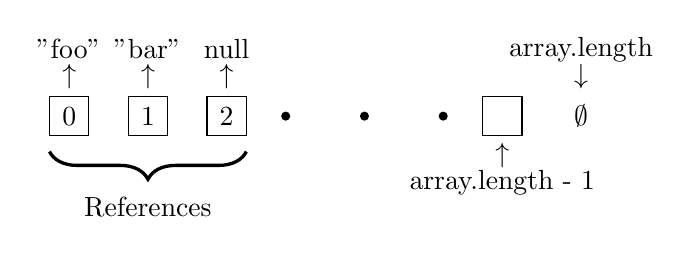
\begin{tikzpicture}
        \foreach \i in {0, 1, ..., 2}
        {
            \draw (\i, 0) rectangle +(0.5, 0.5)
                  node [midway] {\i};
        }
        \foreach \i in {3, 4, 5}
        {
            \draw [fill=black] (\i, 0.25) circle [radius=0.05cm];
        }

        % Objects
        \draw (0.25, 0.75) node {$\uparrow$};
        \draw (0.25, 1.1) node {\lstinline{"foo"}};

        \draw (1.25, 0.75) node {$\uparrow$};
        \draw (1.25, 1.1) node {\lstinline{"bar"}};

        \draw (2.25, 0.75) node {$\uparrow$};
        \draw (2.25, 1.1) node {\lstinline{null}};

        % last valid
        \draw (5.5, 0) rectangle +(0.5, 0.5);
        \draw (5.75, -0.25) node {$\uparrow$};
        \draw (5.75, -0.6) node {\lstinline{array.length - 1}};

        % one-passed-the-end
        \draw (6.75, 0.25) node {$\emptyset$};
        \draw (6.75, 0.75) node {$\downarrow$};
        \draw (6.75, 1.1) node {\lstinline{array.length}};

        \draw [decorate,decoration={brace,amplitude=10pt, mirror}, very thick]
              (0, -0.2) -- (2.5, -0.2);
        \draw (1.25, -0.9) node {References};
    \end{tikzpicture}
    \end{figure}
\end{slide}

\begin{frame}
    \frametitle{Arrays: Initialization}
    \begin{itemize}
        \item Method 1: Allocate inline and fill out-of-line:
              \lstinline{int[] array = new int[5]}
        \item Method 2: Direct initialization:
              \lstinline{int[] array = new int[]\{1, 2, 3, 4, 5\}}
        \item Method 3: Very direct initialization:
              \lstinline{int[] array = \{1, 2, 3, 4, 5\}}
        \item Items are value-initialized:
            \begin{itemize}
                \item \lstinline{int} $\rightarrow$ \lstinline{0}
                \item \lstinline{boolean} $\rightarrow$ \lstinline{false}
                \item \lstinline{double} $\rightarrow$ \lstinline{0.0}
            \end{itemize}
    \end{itemize}
\end{frame}

\begin{frame}[fragile]
    \frametitle{Arrays: Multidimensional}
    \begin{itemize}
        \item Multidimensional arrays possible: \lstinline{int[][][][][] lol = new int[2][3][4][5][6]}
        \item Ragged arrays: arrays with varying dimension
        \begin{lstlisting}
            int[][] ragged = new int[2][];

            ragged[0] = new int[4];
            ragged[1] = new int[123];
        \end{lstlisting}
    \end{itemize}
\end{frame}

\end{document}
